%!TEX root=../GaugeCNNTheory.tex


\subsection{کانولوشن‌های سطحی راهبری‌پذیر-دورانی}
\label{sec:so2_surface_conv}

در این بخش، ما کانولوشن‌های سطحی $\SO2$-، $\CN$- و $\DN$-راهبری‌پذیر را که در ردیف‌های (۳۷-۴۰) جدول~\ref{tab:network_instantiations} فهرست شده‌اند، مرور می‌کنیم.
همه این مدل‌ها در این مشترک هستند که به ابهام جهات مرجع روی سطوح عمومی از طریق یک طراحی هموردای (یا ناوردای) دورانی محلی می‌پردازند، که آنها را از مدل‌های $\{e\}$-راهبری‌پذیر مورد بحث در بخش بعدی~\ref{sec:e_surface_conv} متمایز می‌کند.
قبل از بحث دقیق در مورد مدل‌های منفرد، ما با یک نمای کلی سطح بالا از انتخاب‌های طراحی رایج و گسسته‌سازی‌های عددی ممکن شروع می‌کنیم.


\paragraph{ملاحظات کلی و نمای کلی:}
تمام مدل‌هایی که در این بخش مرور می‌شوند، روی \emph{مش‌های سطحی مثلثی} عمل می‌کنند و راهبری‌پذیر-دورانی هستند.
گروه ساختاری پیوسته $G=\SO2$ برای تمام مدل‌هایی که نمایش‌های میدان منظم را فرض می‌کنند (ردیف‌های (۳۸) و (۳۹)) با گروه‌های دوری~$\CN$ یعنی $N$ جهت با فواصل مساوی، گسسته‌سازی می‌شود.
مدل \citet{huang2019texturenet} یک گروه ساختاری خاص‌تر $\operatorname{D}_4$ را فرض می‌کند.
توجه داشته باشید که معماری‌های صرفاً راهبری‌پذیر-دورانی فقط روی \emph{سطوح جهت‌پذیر} عمل می‌کنند بدون اینکه همواری (پیوستگی) استنتاج خود را نقض کنند.
سطوح غیر جهت‌پذیر نیازمند راهبری‌پذیری بازتابی اضافی هستند، یعنی گروه‌های ساختاری $\O2$ یا $\DN$.
این الزام اغلب با تطبیق‌های جزئی، مهمتر از همه با استفاده از فضاهای کرنل محدودتر، به راحتی قابل ارضا است.


مطابق با تعریف کانولوشن‌های $\GM$, مدل‌ها ویژگی‌ها را در همسایگی محلی اطراف هر نقطه نمونه‌برداری بر حسب \emph{مختصات نرمال ژئودزیک} پارامتری می‌کنند.
تقریباً تمام مدل‌ها میدان‌های ویژگی را روی \emph{رئوس مش} نمونه‌برداری می‌کنند؛ فقط \citet{huang2019texturenet} ویژگی‌ها را به صورت متراکم روی وجوه مش نمونه‌برداری می‌کند.
انتگرال کانولوشن پیوسته در معادله~\eqref{eq:gauge_conv_coord_expression}، که ویژگی‌ها را در مختصات نرمال ژئودزیک با یک کرنل راهبری‌پذیر تطبیق می‌دهد، را می‌توان به روش‌های مختلفی گسسته‌سازی کرد.
اکثر مدل‌ها این انتگرال را در یک رأس $p\in\mathcal{V}$ به عنوان یک جمع روی رئوس همسایه آن $\mathcal{N}_p \subset \mathcal{V}$ گسسته‌سازی می‌کنند.
سپس ویژگی‌ها از این رئوس $q\in\mathcal{N}_p$ با مقادیر کرنل پیوسته در نقطه $\psiTMp \log_p(q) \in \R^2$ تطبیق داده می‌شوند، که در آن $\psiTMp^A$ پیمانه متناظر با چارچوب مرجع انتخاب شده در~$p$ است.
این به همراه انتقال از $q$ به $p$ منجر به گسسته‌سازی زیر می‌شود:
\begin{align}\label{eq:mesh_conv_neighbor_log_discretization}
    \fout^A(p)\ =\ \sum_{q\in\mathcal{N}_p} \textup{A}_q\, K\big(\psiTMp^A \log_p(q)\big)\, \rho\big( g^{A\widetilde{A}}_{p\leftarrow q} \big)\, \fin^{\widetilde{A}}(q) \,,
\end{align}
که در آن $\textup{A}_q \in \R$ وزن‌های مساحتی مناسب انتخاب شده‌اند که مجموع آنها برابر با کل مساحت مش است، ${\sum_{q\in\mathcal{V}} \textup{A}_q = \int_M 1 dp}$.
انتخاب‌های رایج، وزن‌های مساحتی مرکزوار به شکل
\begin{align}\label{eq:triangle_area_weights}
    w_q = \frac{1}{3} \sum_{\{i,j,q\}\in\mathcal{F}} A_{\{i,j,q\}} \,,
\end{align}
هستند، با مجموعی که روی تمام مثلث‌های مجاور رأس~$q$ اجرا می‌شود، یا مساحت‌های ورونوی~\cite{vouga2014lectures}.
از آنجا که گسسته‌سازی در معادله~\eqref{eq:mesh_conv_neighbor_log_discretization} روی رئوس همسایه جمع می‌شود، الگوریتم‌ها نگاشت‌های لگاریتمی را از طریق \emph{کوتاه‌ترین ژئودزیک‌ها} بین $q$ و~$p$ محاسبه می‌کنند؛ به بخش~\ref{sec:surfaces_geom_mesh} و~\cite{polthier1998straightest} مراجعه کنید.

به جای محاسبه نگاشت‌های لگاریتمی رئوس همسایه، می‌توان به طور جایگزین انتگرال کانولوشن را روی دامنه کرنل~$\R^2$ گسسته‌سازی کرد.
نویسندگان \cite{masci2015geodesic} از یک تقسیم‌بندی هم‌زاویه و هم‌شعاع از مختصات قطبی ژئودزیک استفاده می‌کنند.
آنها نگاشت نمایی را برای هر نقطه نمونه‌برداری $(r,\varphi)$ محاسبه می‌کنند، یعنی یک \emph{مستقیم‌ترین ژئودزیک} (\cite{polthier1998straightest}) به طول $r$ را در جهت $\varphi$ نسبت به چارچوب مرجع شلیک می‌کنند.
از آنجا که این ژئودزیک‌ها به طور کلی در یک وجه به پایان می‌رسند، بردارهای ویژگی از رئوس مجاور باید درون‌یابی شوند،
به عنوان مثال بر اساس مختصات مرکزوار.
\citet{Yang2020parallelFrameCNN} همسایگی ژئودزیک را از طریق یک الگوریتم «باز کردن انتقال موازی» تقریب می‌زنند~\cite{budninskiy2018parallel}.


جدول~\ref{tab:network_instantiations} مدل‌ها را بر اساس \emph{انواع میدان} مربوطه خود سازماندهی می‌کند، یعنی بر اساس نمایش‌های گروهی $\rho$ که قوانین تبدیل آنها را تحت تبدیلات پیمانه مشخص می‌کنند.
تنها انواع میدان غیربدیهی که تاکنون استفاده شده‌اند، \emph{نمایش‌های تحویل‌ناپذیر} (مختلط) از $\SO2$ \cite{Wiersma2020} و \emph{نمایش‌های منظم} از $\SO2$ هستند، که با نمایش‌های منظم یک زیرگروه گسسته $\operatorname{C}_N$ گسسته‌سازی شده‌اند~\cite{poulenard2018multi,sun2018zernet,deHaan2020meshCNNs,Yang2020parallelFrameCNN}.
نمایش‌های منظم $\SO2$ بنا به تعریف بر روی توابع در $L^2(\SO2)$ عمل می‌کنند، یعنی بر روی ویژگی‌هایی که «یک مقدار برای هر جهت» اختصاص می‌دهند.
در نسخه گسسته، ما $L^2(\operatorname{C}_N) \cong \R^{|\operatorname{C}_N|} = \R^N$ را داریم، که در آن هر یک از $N$~بعد یک بردار ویژگی منظم متناظر با یکی از جهات در~$\big\{ k\frac{2\pi}{N} \big|\, k=0,\dots,N-1 \big\}$ است.
تناظر با نمایش‌های منظم در اکثر این مقالات ضمنی است -- معماری‌های شبکه بیشتر از یک دیدگاه شهودی‌تر استخراج شده‌اند.
مشخص می‌شود که نویسندگان فقط از زیرمجموعه‌ای از فضای کامل کرنل‌های راهبری‌پذیر که بین میدان‌های ویژگی منظم $\operatorname{C}_N$ نگاشت انجام می‌دهند، استفاده می‌کنند.
ما این ادعا را در ادامه هنگام بحث دقیق در مورد مدل‌ها بیشتر اثبات می‌کنیم.
یک ساختار از فضای کامل کرنل در \cite{Weiler2019_E2CNN} ارائه شده است، یک تصویرسازی را می‌توان در شکل ۳ از~\cite{Weiler2018SFCNN} یافت.
مدل‌های باقی‌مانده بر اساس \emph{نمایش‌های بدیهی}، یعنی \emph{میدان‌های اسکالر} هستند.
یک رویکرد برای محاسبه میدان‌های اسکالر، اعمال یک کرنل در $N$ جهت است، که منجر به یک میدان ویژگی منظم میانی $\operatorname{C}_N$ می‌شود، و به دنبال آن یک عملیات تجمیع روی $N$ پاسخ انجام می‌شود~\cite{masci2015geodesic,monti2017geometric,sun2018zernet}.
از آنجا که تبدیلات پیمانه در $\operatorname{C}_N$ منجر به یک جابجایی دوری صرف (یک جایگشت) از کانال‌های جهت ویژگی می‌شوند، عملیات تجمیع تحت تبدیلات پیمانه \emph{ناوردا} هستند، یعنی میدان‌های اسکالر تولید می‌کنند.
\citet{huang2019texturenet} بلافاصله از کرنل‌های $\operatorname{D}_4$-ناوردا استفاده می‌کند؛ به شکل~\ref{fig:3x3_D4_invariant_kernel} مراجعه کنید.
از آنجا که تبدیلات پیمانه چنین کرنل‌هایی را ناوردا باقی می‌گذارند، میدان‌های ویژگی حاصل نیز ناوردا هستند، یعنی میدان‌های اسکالر.


در آخر، می‌توانیم مدل‌ها را بر اساس \emph{انتقال‌دهنده‌های ویژگی} که فرض می‌کنند، مقایسه کنیم.
تمام شبکه‌های کانولوشنی در \cite{Wiersma2020,poulenard2018multi,sun2018zernet,deHaan2020meshCNNs} انتقال‌دهنده‌های کانونی \emph{لوی-چیویتا} را روی مش فرض می‌کنند.
از آنجا که تمام مدل‌های \cite{masci2015geodesic,monti2017geometric,sun2018zernet,huang2019texturenet} بر \emph{میدان‌های اسکالر} تکیه دارند، انتقال موازی آنها بدیهی است.
یک رویکرد جایگزین توسط \citet{Yang2020parallelFrameCNN} دنبال شد که یک اتصال با مقادیر $\operatorname{C}_N$ را روی مش محاسبه می‌کنند.
این اتصال در همه جا به جز در چند تکینگی با هولونومی $k\frac{2\pi}{N}$ برای یک $k=0,\dots,N-1$ و $N$ ثابت، بدیهی (تخت) است.
نویسندگان اتصال با مقادیر $\operatorname{C}_N$ خود را به گونه‌ای بهینه‌سازی می‌کنند که اتصال لوی-چیویتا با مقادیر $\SO2$ را تا حد امکان نزدیک تقریب بزند؛ همچنین به~\cite{craneTrivialConnectionsDiscrete2010} مراجعه کنید.
توجه داشته باشید که این رویکرد مشابه پهن کردن محلی \lr{CNN}های کروی به \lr{CNN}های بیست‌وجهی ($N=6$) از بخش~\ref{sec:spherical_CNNs_icosahedral} است اما برای مش‌های عمومی اعمال می‌شود.




با در نظر گرفتن این ملاحظات کلی، ما بر روی برخی از انتخاب‌های طراحی خاص‌تر که در مدل‌ها انجام شده است، تمرکز می‌کنیم.


\paragraph{شبکه‌های هارمونیک سطحی:}
\emph{شبکه‌های هارمونیک سطحی} توسط \citet{Wiersma2020} که در ردیف (۳۷) جدول~\ref{tab:network_instantiations} فهرست شده‌اند،
یک مثال نمونه از کانولوشن‌های $\GM$ روی مش‌ها هستند.
آنها شبکه‌های هارمونیک \cite{Worrall2017-HNET} را -- که ویژگی‌های آنها مطابق با نمایش‌های تحویل‌ناپذیر مختلط $G=\SO2$ تبدیل می‌شوند -- از صفحه اقلیدسی به فضاهای خمیده عمومی تعمیم می‌دهند.
نویسندگان کانولوشن خود را مانند معادله~\eqref{eq:mesh_conv_neighbor_log_discretization} با استفاده از وزن‌های مساحتی مرکزوار از معادله~\eqref{eq:triangle_area_weights} تعریف می‌کنند.
انتقال‌دهنده‌های لوی-چیویتا و نگاشت‌های لگاریتمی از طریق روش گرمای برداری~\cite{Sharp2019VectorHeatMethod} محاسبه می‌شوند، که به مش‌های مثلثی محدود نیست بلکه اجازه می‌دهد مدل را به مش‌های چندضلعی و ابرهای نقطه نیز اعمال کرد.
غیرخطی‌های $\SO2$-هموردای مورد استفاده توسط مدل‌ها فقط بر روی قدر مطلق ویژگی‌های مختلط عمل می‌کنند اما آرگومان آنها را ناوردا باقی می‌گذارند.

همانطور که در \cite{lang2020WignerEckart,Weiler2019_E2CNN} اثبات شده است، فضاهای کرنل $\SO2$-راهبری‌پذیر که توسط نویسندگان استفاده می‌شوند، روی میدان مختلط کامل هستند.
با این حال، اگر میدان‌های ویژگی مختلط بر حسب دو کانال که حاوی بخش‌های حقیقی و موهومی آنها هستند، پیاده‌سازی شوند، باید آنها را به عنوان تبدیل شونده مطابق با نمایش‌های تحویل‌ناپذیر حقیقی~$\SO2$ در نظر گرفت.
محدودیت کرنل در این حالت به کرنل‌های راهبری‌پذیر اضافی اجازه می‌دهد؛ برای یک بحث دقیق به پیوست~F.5 از~\cite{Weiler2019_E2CNN} مراجعه کنید.
ما علاوه بر این می‌خواهیم اشاره کنیم که شواهد تجربی نشان می‌دهد که شبکه‌های مبتنی بر میدان‌های نمایش تحویل‌ناپذیر عملکرد به طور قابل توجهی بدتری نسبت به آنهایی که بر اساس نمایش‌های منظم هستند، دارند؛ به عنوان مثال به بنچمارک در~\cite{Weiler2019_E2CNN} مراجعه کنید.
توجه داشته باشید که شبکه‌های هارمونیک سطحی را می‌توان به راحتی با استفاده از «غیرخطی منظم» از~\cite{deHaan2020meshCNNs} که اساساً یک تبدیل فوریه از پشته‌ای از میدان‌های نمایش تحویل‌ناپذیر را برای تبدیل آنها به یک میدان ویژگی منظم اعمال می‌کند، به شبکه‌هایی که روی میدان‌های ویژگی منظم عمل می‌کنند، تبدیل کرد.


\begin{figure}
    \centering
    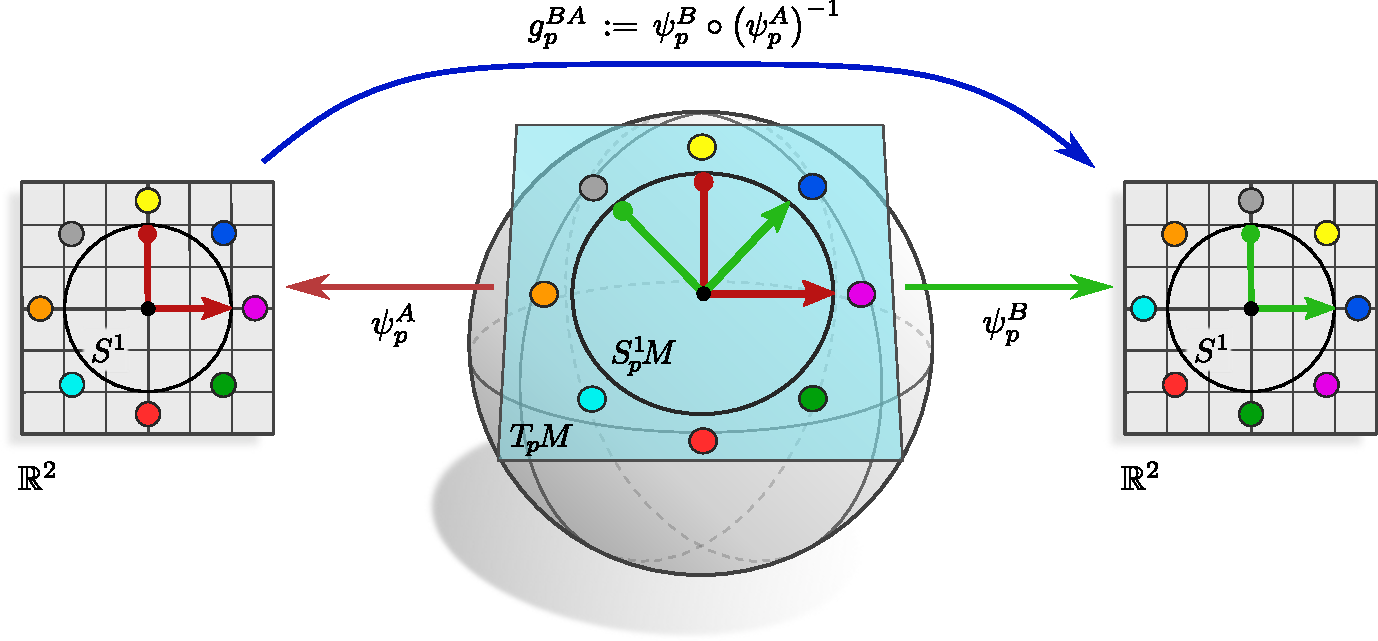
\includegraphics[width=1.\textwidth]{figures/directional_function.pdf}
    \caption{\small
        نمایش \emph{توابع جهتی} توسط \citet{poulenard2018multi}.
        توابع جهتی یک پاسخ با مقدار حقیقی (نقاط رنگی) را به هر جهت (بردار واحد) در $\SpM \subset \TpM$ (دایره سیاه) اختصاص می‌دهند.
        هنگام بیان این توابع نسبت به چارچوب‌های مرجع راست‌هنجار و راست‌گرد یا پیمانه‌های $\psiTMp^X$، نمایش‌های مختصاتی پاسخ‌های با مقدار حقیقی را به بردارهای واحد در $S^1 \subset \R^2$ اختصاص می‌دهند.
        قانون تبدیل بین این نمایش‌های مختصاتی با یک دوران از مقادیر ویژگی روی~$S^1$ داده می‌شود.
        از نظر ریاضی، این قانون تبدیل به عنوان عمل \emph{نمایش منظم} از $\SO2$ شناسایی می‌شود؛ به معادله~\eqref{eq:directional_functions_trafo_law_regular} مراجعه کنید.
        بنابراین توابع جهتی، میدان‌های ویژگی منظم هستند و \lr{CNN} سطحی \citet{poulenard2018multi} بر اساس کانولوشن‌های $\GM$ بین چنین میدان‌هایی است.
        یک نسخه نموداری از این شکل در معادله~\eqref{cd:directional_function_trafo_law} ارائه شده است.
    }
    \label{fig:directional_function}
\end{figure}


\paragraph{\lr{CNN}های ژئودزیک چندجهته:}
\citet{poulenard2018multi} \emph{\lr{CNN}های ژئودزیک چندجهته} (MDGCNNs) را پیشنهاد کردند که روی به اصطلاح \emph{توابع جهتی} عمل می‌کنند.
همانطور که در ادامه استدلال می‌کنیم، توابع جهتی معادل میدان‌های ویژگی منظم هستند و \lr{MDGCNN}ها کانولوشن‌های $\GM$ خاصی بین چنین ویژگی‌هایی هستند.
نویسندگان توابع جهتی را به عنوان توابع با مقدار حقیقی تعریف می‌کنند که به نقاط $p\in M$ و جهات واحد $v\in\TpM,\ \lVert v\rVert=1$ بستگی دارند.
با نشان دادن دایره جهات واحد در $\TpM$ با
\begin{align}
    \SpM\ :=\ \big\{ v\in\TpM \,\big|\, \lVert v\rVert = 1 \big\} \ \ \cong\ \ S^1 \,,
\end{align}
یک ویژگی جهتی در $p$ به عنوان یک نگاشت
\begin{align}
    \digamma: \SpM \to \R
\end{align}
از جهات واحد در صفحه مماس به پاسخ‌های با مقدار حقیقی تعریف می‌شود.%
\footnote{
    تابع جهتی کامل سپس می‌تواند به عنوان یک نگاشت از ${S^1\!M}$، کلافی با تارهای $\SpM$، به مقادیر حقیقی تعریف شود.
}
یک انتخاب از چارچوب مرجع راست‌هنجار و راست‌گرد، یک جهت مرجع را ثابت می‌کند که نسبت به آن می‌توان تابع جهتی را بیان کرد.
فرض کنید~$\psiTMp^A$ پیمانه متناظر با یک چارچوب انتخاب شده باشد، که جهات واحد را در $\SpM \subset \TpM$ به «جهات واحد مختصاتی» در $S^1 \subset \R^2$ نگاشت می‌دهد.
سپس عبارت مختصاتی تابع جهتی با
\begin{align}\label{eq:directional_functions_trafo_law_regular}
    \digamma_p^A\ :=\ \digamma \circ \big(\psiTMp^A \big|_{\SpM} \big)^{-1}\ :\ S^1 \to \R \,,
\end{align}
داده می‌شود، یعنی به بردارهای ضریب واحد روی $\R^2$ پاسخ‌های با مقدار حقیقی اختصاص می‌دهد.
از جابجایی نمودار
\begin{equation}\label{cd:directional_function_trafo_law}
\begin{tikzcd}[column sep=60, row sep=32, font=\normalsize]
    \R^2 \supset S^1
        \arrow[rr, rounded corners, to path={ 
            -- ([yshift=5.ex]\tikztostart.north) 
            --node[above, pos=.5]{\small$g_p^{BA} \mkern2mu\cdot$} ([yshift=5.ex]\tikztotarget.north) 
            -- (\tikztotarget.north)
            }]
        \arrow[dr, "\digamma_p^A"']
    & \SpM
        \arrow[d, pos=.4, "\digamma"]
        \arrow[l, pos=.46, "\psiTMp^A \big|_{\SpM}"']
        \arrow[r, pos=.46, "\psiTMp^B \big|_{\SpM}"]
    &  S^1 \subset \R^2
        \arrow[dl, "\digamma_p^B"]
    \\
    & \R
\end{tikzcd}
\end{equation}
می‌توان خواند که عبارات مختصاتی توابع جهتی از قانون تبدیل زیر پیروی می‌کنند:
\begin{align}
    \digamma_p^B\ =\ \digamma_p^A \circ \big(g_p^{BA}\big)^{-1}\ =:\ \rho_\textup{reg}\big( g_p^{BA}\big)\, \digamma_p^A
\end{align}
تساوی دوم، قانون تبدیل بین عبارات مختصاتی را به عنوان عمل نمایش منظم شناسایی می‌کند، که گزاره ما را مبنی بر اینکه توابع جهتی فقط میدان‌های ویژگی منظم هستند، توجیه می‌کند.%
\footnote{
    به طور دقیق، نمایش منظم $\SO2$ بر روی توابع $\SO2 \to \R$ عمل می‌کند.
    با این حال، ما می‌توانیم به طور کانونی چنین توابعی را با توابع روی $S^1$ با یکی گرفتن $(1,0)\in S^1$ با $\{e\}\in\SO2$ یکی بگیریم.
}
شکل~\ref{fig:directional_function} یک تابع جهتی و نمایش‌های مختصاتی آن را نسبت به چارچوب‌های مختلف نشان می‌دهد.

کانولوشن‌های ژئودزیک چندجهته توسط \citet{poulenard2018multi} بین توابع جهتی به روشی مستقل از مختصات با منقبض کردن آنها با کرنل‌های هموردا در یک پارامتری‌سازی ژئودزیک حول هر رأس، نگاشت انجام می‌دهند.
این مشاهده دلالت بر این دارد که این کانولوشن‌ها کانولوشن‌های $\GM$ خاصی بین میدان‌های ویژگی منظم هستند.
یک تفاوت در فرمول‌بندی کانولوشن‌های ژئودزیک چندجهته این است که پول‌بک انتقال‌دهنده آنها کل بردار ویژگی منظم (تابع جهتی) را در امتداد ژئودزیک‌ها منتقل نمی‌کند، بلکه فقط آن پاسخ منفردی را که متناظر با جهت مماس ژئودزیک است، منتقل می‌کند.
به جای تطبیق ویژگی‌های منتقل شده با یک کرنل ماتریسی، کانولوشن‌های چندجهته پاسخ منفرد منتقل شده را با یک کرنل اسکالر تطبیق می‌دهند.
معادل بودن هر دو عملیات با تحمیل یک الگوی پراکندگی متناظر بر روی کرنل‌های $\SO2$-راهبری‌پذیر ماتریسی ما، که به طور موثر آن پاسخ‌هایی را که توسط \lr{MDGCNN}ها منتقل نمی‌شوند، صفر می‌کند، بازیابی می‌شود.
در حالی که کانولوشن‌های ژئودزیک چندجهته فقط کانولوشن‌های $\GM$ بین میدان‌های ویژگی منظم هستند، آنها بنابراین از فضای کامل کرنل‌های $G$-راهبری‌پذیر بین میدان‌های ویژگی منظم استفاده نمی‌کنند.
این پراکندگی \lr{MDGCNN}ها را از نظر محاسباتی کارآمد می‌کند، با این حال، هزینه حافظه همان باقی می‌ماند و مشخص نیست که این انتخاب تا چه حد ظرفیت بیانی آنها را محدود می‌کند.

تعداد نامتناهی جهات در $\SO2$ (یا $\SpM$ یا $S^1$) در عمل به $N$ جهت با فواصل مساوی در گروه دوری~$\operatorname{C}_N$ گسسته‌سازی می‌شود، به عنوان مثال ۸ جهتی که در شکل~\ref{fig:directional_function} به تصویر کشیده شده‌اند.
از آنجا که انتقال لوی-چیویتا در امتداد ویژگی‌ها به طور کلی با مقادیر $\SO2$ به جای $\operatorname{C}_N$ است، نویسندگان از یک درون‌یابی خطی بین $N$ جهت گسسته استفاده می‌کنند.

همانطور که در بالا بحث شد، \lr{MDGCNN}ها فقط آن پاسخ‌های خاص از ویژگی‌ها را که متناظر با جهت ژئودزیک خروجی نسبت به چارچوب مرجع محلی در~$p$ هستند، منتقل می‌کنند.
این جهت در مبدأ $v=0 \in \TpM$ تعریف نشده است، که از خود-تعاملی رئوس جلوگیری می‌کند.
نویسندگان این مشکل را با اعمال یک \onexone\ اضافی حل می‌کنند که خود-تعاملی گمشده را دوباره اضافه می‌کند.
همانطور که در بخش~\ref{sec:gauge_1x1} استخراج شد، کرنل‌های \onexone\ باید \emph{درهم‌تننده} باشند تا استقلال از مختصات مدل را حفظ کنند.
این الزام در واقع توسط \lr{MDGCNN}ها برآورده می‌شود%
\footnote{
    مکاتبه شخصی با نویسنده.
}
زیرا ماتریس \onexone\ به گونه‌ای ساخته شده است که کل بردارهای ویژگی منظم را با یک وزن یکسان ترکیب می‌کند به جای اینکه کانال‌های آنها را به طور مستقل ترکیب خطی کند.
این کار با نمایش $m_\textup{in}$ ویژگی منظم $\operatorname{C}_N$ نه به عنوان یک بردار ویژگی ${c=N \!\cdot\! m_\textup{in}}$-بعدی بلکه به عنوان یک آرایه با شکل $(N,m_\textup{in})$ و سپس اعمال یک ماتریس (مشترک) با شکل $(m_\textup{out},m_\textup{in})$ روی آخرین محور که منجر به یک آرایه خروجی با شکل $(N,m_\textup{out})$ می‌شود، پیاده‌سازی می‌شود.








\paragraph{CNNهای چارچوب موازی:}
\emph{\lr{CNN}های چارچوب موازی} (PFCNNs) توسط \citet{Yang2020parallelFrameCNN} بر \emph{$N$-میدان‌های چارچوب جهتی} تکیه دارند، که فقط $G$-ساختارهای $\GM$ برای گروه‌های ساختاری دوری~$G=\operatorname{C}_N$ هستند.
به یاد بیاورید از بحث ما در بالا که این میدان‌ها یک اتصال را کدگذاری می‌کنند که در همه جا به جز در چند تکینگی بدیهی است و برای تقریب اتصال لوی-چیویتا اصلی بهینه‌سازی شده است.
از آنجا که این $G$-ساختار در یک مرحله آفلاین از پیش محاسبه می‌شود، ما در ادامه آن را به عنوان داده شده در نظر می‌گیریم و بر روی کانولوشن واقعی \lr{PFCNN} تمرکز می‌کنیم.
مشخص می‌شود که این عملیات معادل یک کانولوشن $\GM$ بین میدان‌های ویژگی منظم $\operatorname{C}_N$ است، با این حال، دوباره یک الگوی پراکندگی خاص را در کرنل‌ها فرض می‌کند که توسط طراحی شبکه خاص القا می‌شود.

\begin{SCfigure}[2.4]
    \hspace*{-2ex}
    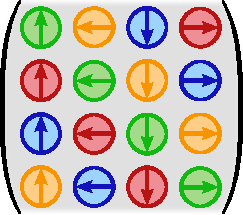
\includegraphics[width=.24\columnwidth]{figures/regular_C4_kernel.pdf}
    \captionsetup{width=1.1\columnwidth}
    \hspace{2ex}
    \caption{\small
        درجات آزادی یک کرنل $\operatorname{C}_N$-راهبری‌پذیر ${K: \R^2 \to \R^{N\times N}}$ که بین میدان‌های ویژگی که مطابق با نمایش منظم ${\rho_{\textup{reg}}: \operatorname{C}_N \to \GL{N}}$ برای $N=4$ تبدیل می‌شوند، نگاشت انجام می‌دهد~\cite{Weiler2019_E2CNN}.
        محدودیت کرنل، معادله~\eqref{eq:kernel_constraint}، الگوی اشتراک وزن با کد رنگی را تحمیل می‌کند.
        \lr{PFCNN}های \citet{Yang2020parallelFrameCNN} ویژگی‌ها را روی هر لایه از $N$-میدان جهتی خود ($\operatorname{C}_N$-ساختار) با نسخه‌های دوران یافته از یک کرنل اسکالر منفرد کانوالو می‌کنند اما شامل تعامل بین لایه‌های مختلف نمی‌شوند.
        این کرنل مشترک متناظر با درایه‌های قطری (سبز) از فضای کامل کرنل است.
        درایه‌های خارج از قطر، که به طور ضمنی مجبور به صفر شدن هستند، متناظر با تعاملات بین لایه‌ها خواهند بود.
    }
    \label{fig:regular_C4_kernel}
\end{SCfigure}

فضاهای ویژگی \lr{PFCNN}ها فضاهای $C^\infty(\GM)$ از توابع با مقادیر حقیقی روی $\GM$ هستند.
از آنجا که $\GM\!\xrightarrow{\piGM}\!M$ برای $G=\operatorname{C}_N$ یک پوشش $|G| = N$-لایه از $M$ است، چنین میدان‌های ویژگی را می‌توان به طور مشابه به عنوان اختصاص یک چندتایی از $N$ عدد حقیقی به هر نقطه~$p\in M$ در نظر گرفت.
از آنجا که $N$ لایه از فضای پوششی علاوه بر این با $N$ جهت (که با اولین محورهای چارچوب داده می‌شوند) یکی گرفته می‌شوند، این ویژگی‌ها معادل توابع جهتی (گسسته‌سازی شده) \citet{poulenard2018multi} هستند.
قضیه~\ref{thm:regular_field_scalar_GM} در پیوست~\ref{apx:regular_field_scalar_GM} علاوه بر این اثبات می‌کند که یک ایزومورفیسم
\begin{align}
    C^\infty(\GM)\ \cong\ \Gamma(\A_{\rho_\textup{reg}})
\end{align}
بین ویژگی‌های \lr{PFCNN}ها و \emph{میدان‌های ویژگی منظم} ما وجود دارد.
بنابراین \lr{PFCNN}ها کانولوشن‌های مستقل از مختصات را بین (معادل) میدان‌های ویژگی منظم انجام می‌دهند و بنابراین به عنوان کانولوشن‌های $\GM$ منظم (خاص) شناسایی می‌شوند.

فرمول‌بندی کانولوشن‌های چارچوب موازی در نگاه اول به نظر می‌رسد کاملاً با فرمول‌بندی ما متفاوت است:
به جای کانوالو کردن کامل میدان‌های ویژگی منظم $N$-بعدی با یک کرنل ماتریسی $\operatorname{C}_N$-راهبری‌پذیر ${K: \R^2 \to \R^{N\times N}}$،
\lr{PFCNN}ها توابع اسکالر خود را روی هر یک از $N$ لایه به طور مستقل با یک کرنل اسکالر مشترک که با چارچوب لایه مربوطه تراز شده است، کانوالو می‌کنند.
این عملیات در چارچوب ما به عنوان یک کانولوشن با یک کرنل ماتریسی $\operatorname{C}_N$-راهبری‌پذیر تفسیر می‌شود که تنها مقادیر غیرصفر آن روی قطر آن قرار دارند و نسبت به یکدیگر چرخانده شده‌اند، که با درایه‌های سبز در شکل~\ref{fig:regular_C4_kernel} به تصویر کشیده شده است.
عدم وجود کوپلینگ بین ویژگی‌ها روی لایه‌های مختلف دلالت بر این دارد که درایه‌های خارج از قطر (زرد، آبی و قرمز) از فضای کامل کرنل راهبری‌پذیر به طور ضمنی صفر در نظر گرفته می‌شوند.
همانطور که قبلاً برای \lr{MDGCNN}ها گفته شد، الگوی پراکندگی این کانولوشن $\GM$ منظم آن را از نظر محاسباتی کارآمدتر از یک کانولوشن $\GM$ متراکم می‌کند اما احتمالاً بر عملکرد آن تأثیر می‌گذارد و هزینه حافظه را کاهش نمی‌دهد.






\begin{figure}
    \centering
    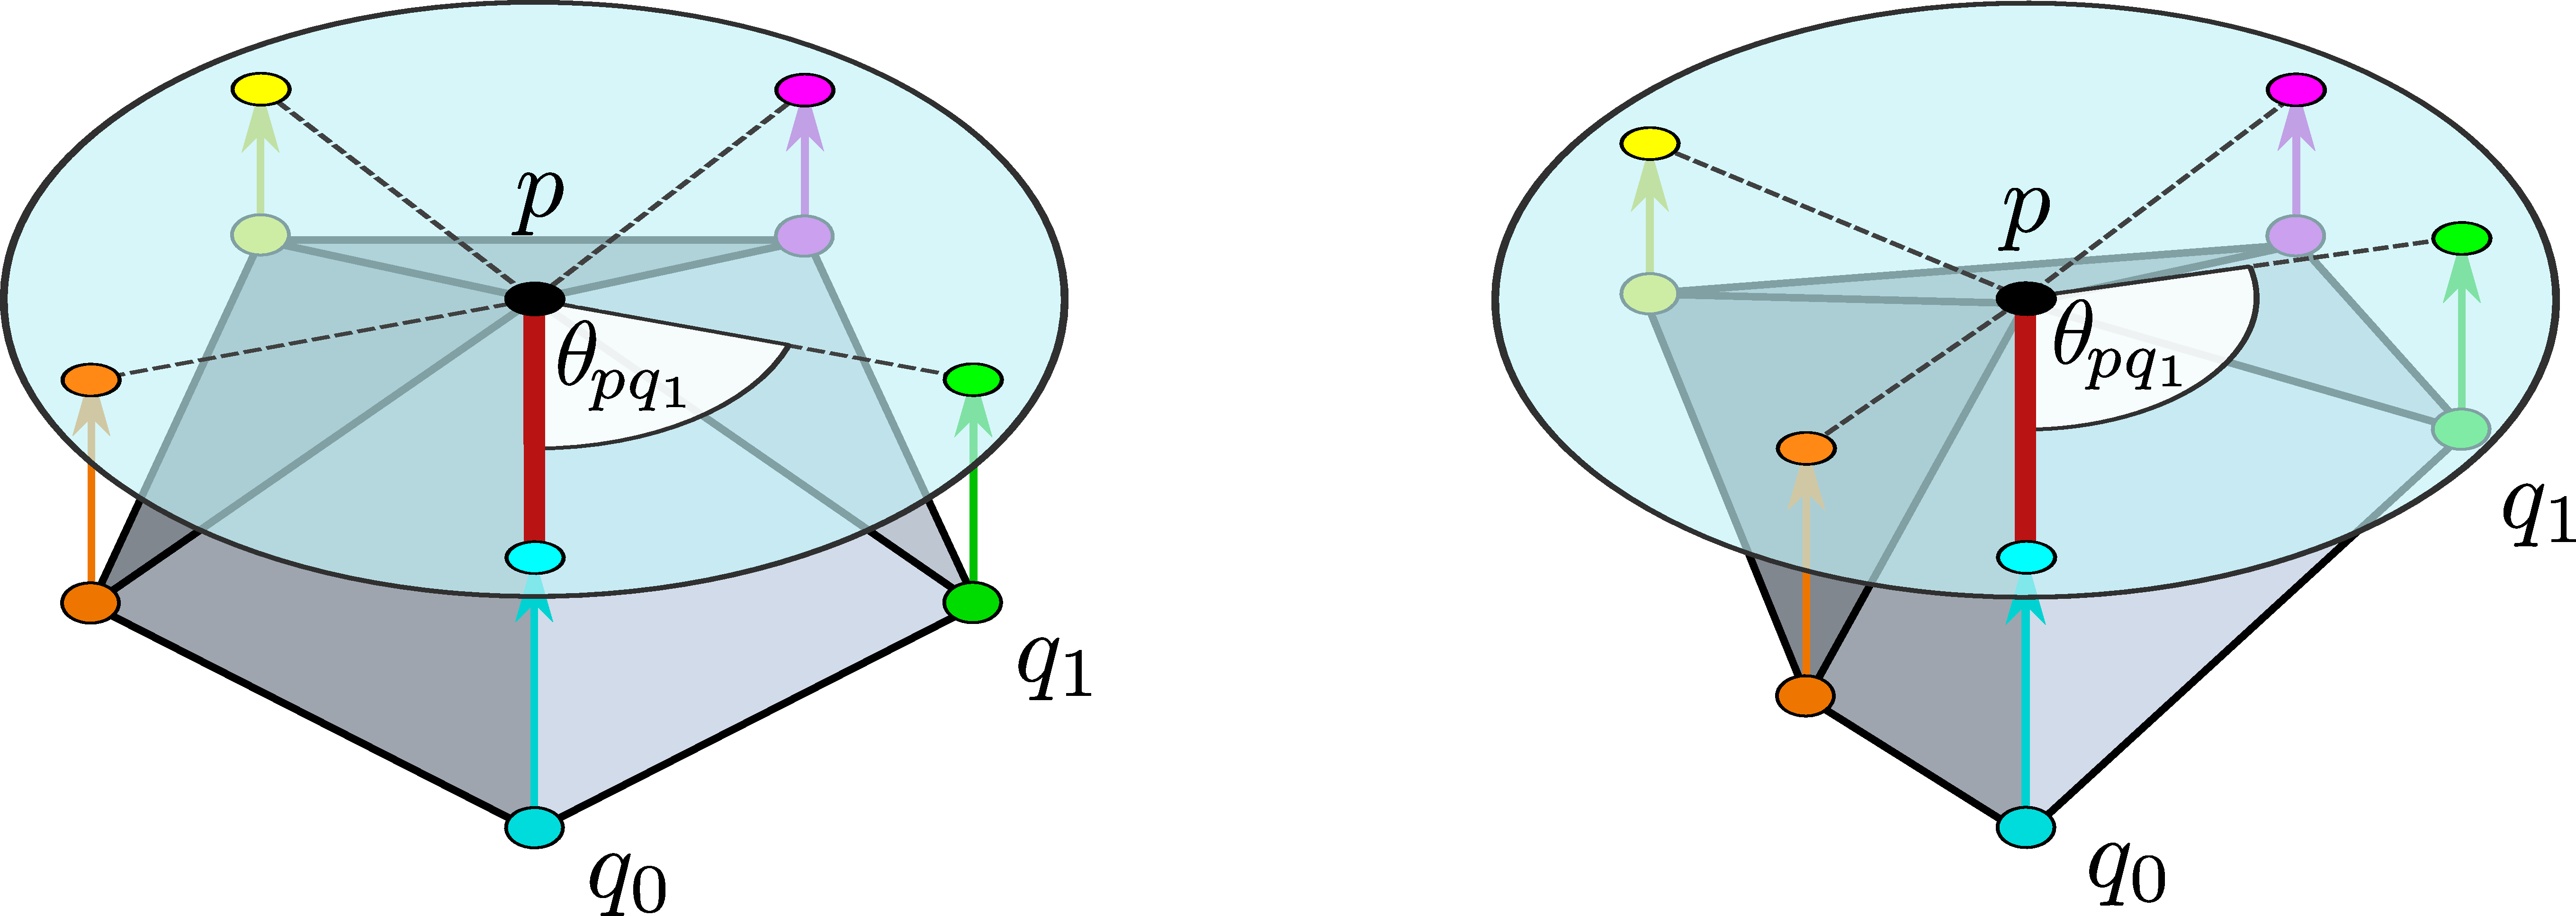
\includegraphics[width=.7\columnwidth]{figures/mesh_CNN_neighborhood_geometry.pdf}
    \vspace*{1ex}
    \caption{\small
        دو ناحیه مش که از نظر توپولوژیکی معادل اما از نظر هندسی متمایز هستند.
        یک رویکرد برای تعریف کانولوشن‌ها روی مش‌ها، در نظر گرفتن گراف زیربنایی آنها $(\mathcal{V},\mathcal{E})$ است که توپولوژی مش را ثبت می‌کند، و اجرای یک شبکه عصبی گراف روی آن.
        شبکه‌های عصبی گراف (متعارف) به دلیل نداشتن اطلاعات در مورد هندسه مش، نمی‌توانند بین دو همسایگی به تصویر کشیده شده تمایز قائل شوند.
        از نظر هندسی، آنها کرنل‌های \emph{همسانگرد} را اعمال می‌کنند.
        \emph{\lr{CNN}های مش هموردای پیمانه} توسط \citet{deHaan2020meshCNNs} این مشکل را با تصویر کردن رئوس همسایه $q_i$ روی صفحات مماس و اختصاص دادن زوایای $\theta_{pq_i}$ به آنها نسبت به یک یال مرجع، یعنی پیمانه (قرمز)، حل می‌کنند.
        الزام به استقلال از مختصات کانولوشن‌ها منجر به کرنل‌های $G$-راهبری‌پذیر می‌شود.
        در حالی که این مدل می‌تواند بر اساس \emph{جهت} گره‌های همسایه تمایز قائل شود، \emph{فاصله} آنها را نادیده می‌گیرد.
        این مدل علاوه بر این از پارامتری‌سازی ژئودزیک ما منحرف می‌شود به این دلیل که تکیه‌گاه کرنل آن بر اساس اتصال لبه محلی به جای فواصل ژئودزیک است.
    }
    \label{fig:mesh_CNNs_neighborhood}
\end{figure}


\paragraph{\lr{CNN}های مش هموردای پیمانه:}
\emph{\lr{CNN} مش هموردای پیمانه} (\lr{GEMCNN}) توسط \citet{deHaan2020meshCNNs} از کاستی‌های شبکه‌های عصبی گراف متعارف برای پردازش میدان‌های ویژگی روی مش‌ها الهام گرفته شده است.
به طور خاص، شبکه‌های عصبی گراف وانیلی می‌توانند برای پردازش میدان‌های ویژگی نمونه‌برداری شده در رئوس روی مش‌ها با کانوالو کردن روی گراف $(\mathcal{V},\mathcal{E})$ که توسط مش القا می‌شود، استفاده شوند.
مشکل این رویکرد این است که گراف فقط \emph{توپولوژی} مش را کدگذاری می‌کند، اما قادر به ثبت \emph{هندسه} آن نیست.
کانولوشن‌های گراف متعارف بر این اساس بین ترتیب یال‌ها تمایز قائل نمی‌شوند، که روی مش‌ها متناظر با استفاده از \emph{کرنل‌های همسانگرد} است که بین میدان‌های اسکالر نگاشت انجام می‌دهند.
شکل~\ref{fig:mesh_CNNs_neighborhood} دو ناحیه از یک مش با هندسه متمایز اما توپولوژی معادل را نشان می‌دهد -- برای کانولوشن‌های گراف متعارف هر دو همسایگی یکسان به نظر می‌رسند.
\lr{GEMCNN}ها این مشکل را با انتخاب یک یال مرجع در هر رأس $p\in\mathcal{V}$ حل می‌کنند، که نسبت به آن جهت تمام یال‌های دیگر $\{p,q_i\} \in\mathcal{E}$ به حلقه یک از همسایگان $q_i\in \mathcal{N}_p \subset\mathcal{V}$ بر حسب زوایا $\theta_{pq_i} \in [0,2\pi)$ اندازه‌گیری می‌شود.
یک انتخاب از یال مرجع متناظر با یک انتخاب از چارچوب راست‌هنجار و راست‌گرد است.
انتخاب‌های مختلف با تبدیلات پیمانه در گروه ساختاری~$G=\SO2$ مرتبط هستند.

همانند نظریه ما، فضاهای ویژگی \lr{GEMCNN}ها به عنوان مقاطعی از کلاف‌های برداری همبسته تعریف می‌شوند، یعنی به عنوان فضاهایی از میدان‌های ویژگی $c$-بعدی که ضرایب آنها تحت تبدیلات پیمانه مطابق با یک نمایش گروهی $\rho: \SO2 \to \GL{c}$ تبدیل می‌شوند.
به هر یال یک انتقال‌دهنده لوی-چیویتا با مقادیر $\SO2$ اختصاص داده می‌شود.
عملیات کانولوشن ملزم است که مستقل از انتخاب یال مرجع باشد، که منجر به الزام بر روی کرنل‌ها برای $G$-راهبری‌پذیر بودن (هموردایی پیمانه) می‌شود.
بر خلاف فرمول‌بندی ما، کرنل‌ها مستقیماً در مختصات نرمال ژئودزیک اعمال نمی‌شوند بلکه پیام‌ها را فقط از همسایگی‌های یک-حلقه $\mathcal{N}_p := \{q\in\mathcal{V} \,|\, \{p,q\}\in\mathcal{E} \}$ به آن گره~$p$ که کرنل حول آن متمرکز است، منتقل می‌کنند.%
\footnote{
    برای یک شبکه (به اندازه کافی) منظم و کرنل با تکیه‌گاه فشرده در مختصات ژئودزیک، هر دو رویکرد معادل می‌شوند.
}
کرنل‌ها علاوه بر این \emph{غیرحساس به شعاع} هستند -- اینکه این تا چه حد بر عملکرد مدل تأثیر می‌گذارد، یک سؤال باز باقی می‌ماند.

نویسندگان \emph{نمایش‌های تحویل‌ناپذیر} (حقیقی) را به عنوان انواع میدان برای کانولوشن انتخاب کرده‌اند، با این حال، آنها یک تغییر پایه به \emph{نمایش‌های منظم} برای اعمال غیرخطی‌های \lr{ReLU} انجام می‌دهند، به همین دلیل ما آنها را در ردیف (۳۸) جدول~\ref{tab:network_instantiations} به جای ردیف (۳۷) فهرست می‌کنیم.%
\footnote{
    معادل بودن میدان‌های-$\rho$ با \emph{تجزیه نمایش تحویل‌ناپذیر} آنها در بخش~\ref{sec:mobius_representations} و در بخش ۲.۴ از~\cite{Weiler2019_E2CNN} مورد بحث قرار گرفت.
}
به طور خاص، نویسندگان از تغییر پایه $Q\in\R^{N\times N}$ استفاده می‌کنند که نمایش منظم $\rho_{\textup{reg}}: \operatorname{C}_N \to \GL{N}$ از $\operatorname{C}_N$ را به مؤلفه‌های نمایش تحویل‌ناپذیر آن تجزیه می‌کند تا یک پشته از میدان‌های نمایش تحویل‌ناپذیر را به یک میدان ویژگی منظم تبدیل کند.
برای $\operatorname{C}_N$ این ماتریس فقط تبدیل فوریه گسسته است.
پس از اعمال غیرخطی \lr{ReLU} به هر یک از $N$ کانال از میدان ویژگی منظم به طور جداگانه -- که یک عملیات $\operatorname{C}_N$-هموردا است زیرا نمایش‌های منظم، نمایش‌های جایگشتی هستند -- ویژگی‌ها برای عملیات کانولوشن بعدی به یک پشته از میدان‌های نمایش تحویل‌ناپذیر بازگردانده می‌شوند.
این طراحی این مزیت را دارد که ویژگی‌ها را می‌توان دقیقاً با انتقال‌دهنده‌های با مقادیر $\SO2$ منتقل کرد، بدون اینکه نیاز به بازگشت به یک طرح درون‌یابی باشد، همانطور که توسط~\citet{poulenard2018multi} انجام می‌شود.
توجه داشته باشید، با این حال، که شبکه کامل به دلیل استفاده از غیرخطی‌های منظم فقط $\operatorname{C}_N$-هموردا است.

اینکه نویسندگان از نمایش‌های تحویل‌ناپذیر \emph{حقیقی} از $\SO2$ استفاده می‌کنند به این معنی است که فضاهای کرنل آنها تقریباً دو برابر بزرگتر از فضاهای کرنل شبکه‌های هارمونیک سطحی توسط \citet{Wiersma2020} است؛ بحث‌ها در~\cite{Weiler2019_E2CNN,lang2020WignerEckart} را مقایسه کنید.



\paragraph{\lr{CNN}های ژئودزیک:}
اولین کار در مورد کانولوشن‌های ژئودزیک که ما از آن آگاه هستیم، کار \citet{masci2015geodesic} است.
نویسندگان ابهام دورانی مختصات قطبی ژئودزیک را روی یک منیفلد ریمانی جهت‌پذیر شناسایی کرده و آن را از طریق یک معماری \emph{ناوردا} نسبت به دوران حل می‌کنند.
\emph{کانولوشن‌های ژئودزیک} آنها یک میدان \emph{اسکالر} را نسبت به مختصات قطبی ژئودزیک با جهت‌گیری دلخواه نمایش می‌دهند.
از آنجا که نوع میدان بدیهی است، پول‌بک انتقال‌دهنده به مختصات ژئودزیک به انتقال‌دهنده‌های (غیربدیهی) نیاز ندارد.
سپس میدان ویژگی در مختصات ژئودزیک با یک کرنل اسکالر تطبیق داده می‌شود، که در $N$ دوران با فواصل مساوی با زوایای $\frac{2\pi}{N}k$ نسبت به چارچوب مرجع، که در آن $k=0,\dots,N-1$ است، اعمال می‌شود.
از آنجا که یک تبدیل پیمانه با $\frac{2\pi}{N}l$ برای یک $l\in\{0,\dots,N-1\}$ تمام کرنل‌ها را بر این اساس می‌چرخاند، منجر به یک جایگشت دوری از پاسخ‌ها با $l$ گام می‌شود.
بنابراین این عملیات در چارچوب ما متناظر با یک کانولوشن $\operatorname{C}_N$-راهبری‌پذیر از میدان‌های اسکالر به میدان‌های ویژگی منظم $\operatorname{C}_N$ است.
به جای پردازش بیشتر این میدان‌ها از طریق کانولوشن‌های گروهی منظم
-- همانطور که در \lr{MDGCNN}ها~\cite{poulenard2018multi}، \lr{PFCNN}ها~\cite{Yang2020parallelFrameCNN} و \lr{GEMCNN}ها~\cite{deHaan2020meshCNNs} انجام می‌شود --
نویسندگان یک عملیات تجمیع $\max$ را روی $N$ پاسخ اعمال می‌کنند.
از آنجا که تبدیلات پیمانه با مقادیر $\operatorname{C}_N$ منجر به جابجایی‌های دوری از میدان‌های ویژگی منظم میانی می‌شوند، عملیات تجمیع ناوردای-پیمانه است، یعنی میدان‌های اسکالر تولید می‌کند.
در حالی که طراحی این شبکه برای پیاده‌سازی ساده است، از کدگذاری اطلاعات جهتی توسط ویژگی‌ها جلوگیری می‌کند.
انواع دیگری از این طراحی شبکه را می‌توان در \cite{masci2015shapenet,monti2017geometric} یافت.







\paragraph{ZerNet:}
در ادامه، به \emph{ZerNet} توسط \citet{sun2018zernet} می‌پردازیم.
برای جلوگیری از سردرگمی، اشاره می‌کنیم که نویسندگان دو مدل را پیشنهاد کرده‌اند، که ما آنها را به ترتیب در ردیف‌های (۳۸) \emph{و} (۳۹) جدول~\ref{tab:network_instantiations} فهرست می‌کنیم.
ما هر دو مدل را با شروع از انتخاب‌های طراحی مشترک آنها توصیف می‌کنیم.

مفهوم کلیدی زیربنای \lr{ZerNet}ها، پارامتری‌سازی کرنل‌های کانولوشن بر حسب \emph{چندجمله‌ای‌های زرنیکه} است، که یک پایه متعامد از توابع را روی دیسک واحد بسته $B_{\R^2}(0,1)$ حول مبدأ $\R^2$ تشکیل می‌دهند.
در مختصات قطبی، چندجمله‌ای‌های زرنیکه با
\begin{alignat}{3}
	\textup{زوج:}\quad&&
		Z_n^m	&:\ [0,1]\times[0,2\pi) \to [-1,1], \quad (r,\varphi) \mapsto R_n^m(r)\, \cos(m\varphi)
		\qquad&& n\in\N,\ \ 0\leq m\leq n \\
	\textup{فرد:}\quad&&
		Z_n^{-m} &:\ [0,1]\times[0,2\pi) \to [-1,1], \quad (r,\varphi) \mapsto R_n^m(r)\, \sin(m\varphi)
		\qquad&& n\in\N,\ \ 1\leq m\leq n \,,
\end{alignat}
داده می‌شوند، که در آن $R_n^m$ چندجمله‌ای‌های شعاعی زرنیکه هستند.
اینکه چندجمله‌ای‌های زرنیکه (که به طور مناسب نرمال‌سازی شده‌اند) راست‌هنجار هستند به این معنی است که آنها روابط راست‌هنجاری
\begin{align}
	\big\langle Z_n^m,\, Z_k^l \big\rangle_{B_{\R^2}(0,1)}
	\ =\ \int_0^1 \int_0^{2\pi} Z_n^m(r,\varphi)\, Z_k^l(r,\varphi)\ r\, dr\, d\varphi
	\ =\ \delta_{nk}\, \delta_{ml} \,.
\end{align}
را برآورده می‌کنند. یک تابع روی دیسک واحد، به عنوان مثال یک کرنل اسکالر $K: B_{\R^2}(0,1) \to \R$، را می‌توان در پایه چندجمله‌ای‌های زرنیکه بسط داد:
\begin{align}
	K(r,\varphi)\ =\ \sum_{n\in\N}\, \sum_{m=-n}^n \widehat{K}_n^m\, Z_n^m(r,\varphi)
\end{align}
برای بازیابی ضرایب بسط یک تابع داده شده روی دیسک واحد، آن را روی پایه زرنیکه تصویر می‌کنیم:
\begin{align}
	\widehat{K}_n^m
	\ =\ \big\langle K,\, Z_n^m \big\rangle_{B_{\R^2}(0,1)}
	\ =\ \int_0^1 \int_0^{2\pi} K(r,\varphi)\, Z_n^m(r,\varphi)\ r\, dr\, d\varphi
\end{align}
حاصلضرب داخلی بین دو تابع $K$ و $\Expspf^A$ روی دیسک واحد را می‌توان با این روابط بر حسب ضرایب بسط آنها بیان کرد:
\begin{align}\label{eq:zernike_kernel_matching}
	\big\langle K,\, \Expspf^A \big\rangle_{B_{\R^2}(0,1)}
	\ =&\ \int_0^1 \int_0^{2\pi} K(r,\varphi)\, \Expspf^A(r,\varphi)\ r\, dr\, d\varphi \notag \\
	\ =&\ \int_0^1 \int_0^{2\pi}
		\sum_{n\in\N}\, \sum_{m=-n}^n \widehat{K}_n^m\, Z_n^m(r,\varphi)\,
		\sum_{k\in\N}\, \sum_{l=-k}^k \widehat{\big[\Expspf^A\big]}_k^l\, Z_k^l(r,\varphi)\ 
		r\, dr\, d\varphi \notag \\
	\ =&\ 
		\sum_{n\in\N}\, \sum_{m=-n}^n 
		\sum_{k\in\N}\, \sum_{l=-k}^k 
		\underbrace{\int_0^1 \int_0^{2\pi}\!
		Z_n^m(r,\varphi)\, Z_k^l(r,\varphi)\ 
		r\, dr\, d\varphi}_{\delta_{nk}\, \delta_{ml}}\ 
		\widehat{K}_n^m\, \widehat{\big[\Expspf^A\big]}_k^l \notag \\
	\ =&\ 
		\sum_{n\in\N}\, \sum_{m=-n}^n 
		\widehat{K}_n^m\, \widehat{\big[\Expspf^A\big]}_n^m
\end{align}
همانطور که با انتخاب‌های $K$ و $\Expspf^A$ برای این توابع پیشنهاد می‌شود، نویسندگان از این ویژگی برای تطبیق کرنل‌ها با پول‌بک میدان‌های ویژگی به مختصات قطبی ژئودزیک استفاده می‌کنند.
ضرایب کرنل $\widehat{K}_n^m$ که فراتر از یک آستانه مشخص شده توسط کاربر صفر می‌شوند، به عنوان پارامترهای یادگرفتنی شبکه بهینه‌سازی می‌شوند.
ضرایب بسط $\widehat{\big[\Expspf^A\big]}_n^m$ از پول‌بک انتقال‌دهنده میدان ویژگی با حل یک سیستم معادلات خطی محاسبه می‌شوند.

یک مزیت پارامتری‌سازی کرنل بر حسب چندجمله‌ای‌های زرنیکه این است که آنها بنا به تعریف \emph{کرنل‌های $\SO2$-راهبری‌پذیر} هستند.
به طور خاص، زوج‌های $\big(Z_n^m, Z_n^{-m}\big)^\top$ از کرنل‌ها برای یک $n\in\N$ و $1\leq m\leq n$ داده شده، یک زوج از کرنل‌ها را تشکیل می‌دهند که با ضرب آنها در نمایش تحویل‌ناپذیر حقیقی مرتبه $m$-ام از~$\SO2$ چرخانده می‌شوند،
\begin{align}
	\begin{pmatrix}
		Z_n^m \\ Z_n^{-m}
	\end{pmatrix}
	(r,\varphi + \Delta\varphi)
	\ =\ 
	\begin{pmatrix}
		\cos(m\Delta\varphi) &         -  \sin(m\Delta\varphi) \\
		\sin(m\Delta\varphi) & \phantom{-} \cos(m\Delta\varphi)
	\end{pmatrix}
	\begin{pmatrix}
		Z_n^m \\ Z_n^{-m}
	\end{pmatrix}
	(r,\varphi) \,,
\end{align}
در حالی که کرنل‌های $Z_n^0$ یعنی برای $m=0$ به طور بدیهی تبدیل می‌شوند (آنها همسانگرد هستند).
توجه داشته باشید که \emph{ضرایب بسط} $\widehat{K}_n^m$ از یک کرنل $K$ به صورت \emph{وارون} نسبت به پایه تبدیل می‌شوند.
نویسندگان از این قانون تبدیل برای دوران تحلیلی کرنل‌ها بر حسب ضرایب بسط آنها استفاده می‌کنند.
راهبری‌پذیری دورانی چندجمله‌ای‌های زرنیکه مستقل از بخش‌های شعاعی آنها است اما به این واقعیت بستگی دارد که بخش‌های زاویه‌ای آنها \emph{هارمونیک‌های دایره‌ای} هستند، که توابع پایه هارمونیک در تجزیه پیتر-ویل از $L^2(\SO2)$ هستند~\cite{lang2020WignerEckart}.
به دلیل ویژگی‌های راهبری‌پذیری آنها، پایه‌های هارمونیک دایره‌ای به طور گسترده برای پارامتری کردن کرنل‌های کانولوشن حقیقی~\cite{Weiler2018SFCNN,graham2020dense} و مختلط~\cite{Worrall2017-HNET,Wiersma2020} حداقل از دهه ۸۰ میلادی استفاده شده‌اند~\cite{Hsu1982optical,Rosen1988circularHarmonic,freeman1991design,hel1998canonical}.
در واقع، هارمونیک‌های دایره‌ای زیربنای \emph{هر} کرنل $\SO2$-راهبری‌پذیر هستند~\cite{Weiler2019_E2CNN,lang2020WignerEckart}.

اولین و اصلی‌ترین طراحی مدل توصیف شده توسط \citet{sun2018zernet} مشابه طراحی \citet{masci2015geodesic} است.
یک میدان اسکالر به مختصات نرمال ژئودزیک پول‌بک می‌شود، جایی که با یک کرنل اسکالر که در $N$ دوران گسسته اعمال می‌شود، تطبیق داده می‌شود، که منجر به یک میدان ویژگی منظم میانی $\operatorname{C}_N$ می‌شود.
یک عملیات تجمیع $\max$ بعدی روی $N$ پاسخ سپس یک خروجی $\operatorname{C}_N$-ناوردا، یعنی یک میدان خروجی اسکالر، به دست می‌دهد.
تفاوت با پیاده‌سازی \citet{masci2015geodesic} این است که این عملیات در پایه چندجمله‌ای‌های زرنیکه همانطور که در معادله~\eqref{eq:zernike_kernel_matching} مشخص شده است، انجام می‌شود.
این انتخاب در نهایت متناظر با یک طرح درون‌یابی جایگزین است.
طراحی مدل دوم، که در بخش ۴.۴ از~\cite{sun2018zernet} توصیف شده است، یک پیاده‌سازی مجدد از \lr{MDGCNN}های \citet{poulenard2018multi} در پایه چندجمله‌ای‌های زرنیکه است.
نویسندگان مشاهده می‌کنند که این طراحی منجر به عملکرد به طور قابل توجهی بهبود یافته‌ای می‌شود زیرا میدان‌های ویژگی منظم قادر به کدگذاری اطلاعات جهتی هستند.





\paragraph{TextureNet:}
آخرین مدل راهبری‌پذیر-دورانی که ما مورد بحث قرار می‌دهیم، \emph{TextureNet} توسط \citet{huang2019texturenet} است.
\begin{wrapfigure}[13]{r}{0.22\textwidth}
    \centering
    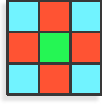
\includegraphics[width=.16\textwidth]{figures/3x3_D4_invariant_kernel.pdf}
    \captionsetup{width=.21\textwidth}
    \caption{\small
        \\
        یک کرنل $3\times3$ پیکسلی $\operatorname{D}_4$-ناوردا با سه درجه آزادی پارامتری می‌شود.
    }
    \label{fig:3x3_D4_invariant_kernel}
\end{wrapfigure}%
بر خلاف مدل‌های قبلی، \lr{TextureNet}ها یک $\operatorname{D}_4$-ساختار را فرض می‌کنند، که به راحتی می‌توان آن را به یک $\operatorname{D}_N$-ساختار تعمیم داد.
این $\operatorname{D}_4$-ساختار با استفاده از \lr{QuadriFlow}، یک بسته نرم‌افزاری شخص ثالث که می‌تواند برای محاسبه میدان‌های ۴-RoSy که برای هموار بودن و داشتن تکینگی‌های کم بهینه شده‌اند، استفاده شود، از پیش محاسبه می‌شود~\cite{Huang2018QuadriFlow}.
همانطور که از نام آن پیداست، \lr{TextureNet}ها میدان‌های ویژگی ورودی را که به عنوان بافت نمایش داده می‌شوند، پردازش می‌کنند و دارای وضوح بالقوه بالاتری نسبت به مش هستند.
کرنل‌های کانولوشن در یک مجموعه متراکم از مکان‌های نمونه‌برداری، که به طور یکنواخت روی وجوه مش توزیع شده‌اند، اعمال می‌شوند.
در هر نقطه نمونه‌برداری، میدان ویژگی اسکالر به مختصات نرمال ژئودزیک پول‌بک شده و نسبت به یک چارچوب دلخواه از $\operatorname{D}_4$-ساختار نمایش داده می‌شود.
سپس با یک کرنل $3\times3$ $\operatorname{D}_4$-ناوردا تطبیق داده می‌شود.
همانطور که در شکل~\ref{fig:3x3_D4_invariant_kernel} به تصویر کشیده شده است، ۹ پیکسل از چنین کرنل‌هایی با ۳ درجه آزادی توصیف می‌شوند.
کانولوشن بر حسب سه \onexone\ پیاده‌سازی می‌شود که پاسخ‌های آنها متعاقباً در هر یک از فضاهای مماس تقسیم‌بندی و agregaste می‌شوند.
راهبری‌پذیری بازتابی اضافی کرنل‌ها دلالت بر این دارد که \lr{TextureNet}ها روی سطوح غیرجهت‌پذیر به خوبی تعریف شده‌اند.
با این حال، از آنجا که ویژگی‌های \lr{TextureNet} میدان‌های اسکالر هستند، نمی‌توانند نه جهات و نه جهت‌گیری‌ها را کدگذاری کنند.
برای غلبه بر این مشکل، لازم است از کرنل‌های $\operatorname{D}_N$ یا $\O2$-راهبری‌پذیر غیربدیهی استفاده شود.